\documentclass[a4paper,11pt]{report}

% Required packages
\usepackage[utf8]{inputenc}
\usepackage[T1]{fontenc}
\usepackage{lmodern}
\usepackage[english]{babel}
\usepackage{graphicx}
\usepackage{xcolor}
\usepackage{hyperref}
\usepackage[most]{tcolorbox}
\usepackage{enumitem}
\usepackage{fancyhdr}
\usepackage[margin=2.5cm, headheight=14pt]{geometry}
\usepackage{minted}
\usepackage{fontawesome5}
\usepackage{dirtree}

% Hyperref configuration
\hypersetup{
    colorlinks=true,
    linkcolor=blue,
    filecolor=magenta,
    urlcolor=blue,
    pdftitle={OSCam Connection Manager - User Guide},
    pdfpagemode=FullScreen,
    bookmarksopen=true
}

% Custom styles for boxes with lighter colors
\newtcolorbox{tipbox}[1][]{
    enhanced,
    colback=green!15!white,
    colframe=green!50!black,
    title={\faLightbulb\ Tip},
    fonttitle=\bfseries\color{black},
    sharp corners,
    boxrule=1pt,
    #1
}

\newtcolorbox{warningbox}[1][]{
    enhanced,
    colback=pink!15!white,
    colframe=red!45!black,
    title={\faExclamationTriangle\ Warning},
    fonttitle=\bfseries\color{black},
    sharp corners,
    boxrule=1pt,
    #1
}

\newtcolorbox{procedurebox}[1][]{
    enhanced,
    colback=cyan!10!white,
    colframe=cyan!60!black,
    title={\faList\ Procedure},
    fonttitle=\bfseries\color{black},
    sharp corners,
    boxrule=1pt,
    #1
}

\newtcolorbox{notebox}[1][]{
    enhanced,
    colback=yellow!15!white,
    colframe=yellow!50!black,
    title={\faInfoCircle\ Note},
    fonttitle=\bfseries\color{black},
    sharp corners,
    boxrule=1pt,
    #1
}

% Header and footer configuration
\pagestyle{fancy}
\fancyhf{}
\fancyhead[L]{OSCam Connection Manager}
\fancyhead[R]{User Guide}
\fancyfoot[C]{\thepage}
\renewcommand{\headrulewidth}{0.4pt}
\renewcommand{\footrulewidth}{0.4pt}

\begin{document}

% Added PDF metadata
\pdfinfo{
  /Title (OSCam Connection Manager - User Guide)
  /Author (mapi68)
  /Subject (User Guide for OSCam Connection Manager)
  /Keywords (OSCam, FTP, configuration management)
}

\begin{titlepage}
    \centering
    \vspace*{2cm}
    
\includegraphics[width=0.3\textwidth]{icon.png}\par\vspace{1cm}
    {\Huge\bfseries OSCam Connection Manager\\[0.5cm]}
    {\large\bfseries User Guide\\[2cm]}
    {\large Version 1.0\\[1cm]}
    {\large \today\\[2cm]}
    \vfill
    {\large A graphical tool for managing OSCam configurations\\through FTP connections developed by mapi68}\\[0.5cm]
    {\large \url{https://github.com/mapi68/oscam-connection-manager}}\\[1cm]
    {\large Copyright © 2024 - All rights reserved}
\end{titlepage}

\tableofcontents
\newpage

\chapter{Introduction}

\section{About OSCam Connection Manager}
OSCam Connection Manager is a graphical tool designed to help you manage OSCam configurations across multiple servers using FTP connections. It provides an intuitive dark-themed interface for:
\begin{itemize}
    \item Managing multiple OSCam server connections via FTP
    \item Viewing and editing oscam.server configurations
    \item Creating manual backups of OSCam configurations
    \item Restarting OSCam services remotely
\end{itemize}

\begin{figure}[!htb]
    \centering
    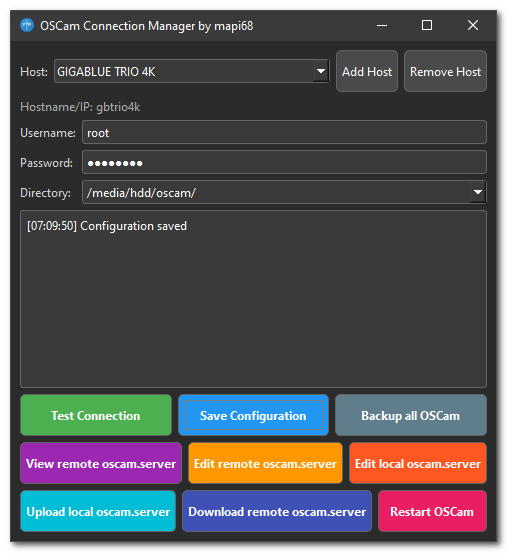
\includegraphics[width=0.8\textwidth]{screenshot.png}
    \caption{OSCam Connection Manager Main Interface}
    \label{fig:main-interface}
\end{figure}

\section{Key Features}
\begin{itemize}
    \item \textbf{Multi-Server Support}: Manage multiple OSCam servers from a single interface
    \item \textbf{Dark Theme Interface}: Modern, eye-friendly dark theme
    \item \textbf{Manual Backup System}: Create backups of your OSCam configurations on demand
    \item \textbf{Remote Control}: Restart OSCam services through web interface
    \item \textbf{File Management}: View, edit, and transfer configuration files via FTP
\end{itemize}

\chapter{Installation}

\section{System Requirements}
\begin{procedurebox}
\textbf{Essential Requirements:}
\begin{itemize}
    \item Python 3.6 or higher
    \item FTP access to your OSCam server(s)
    \item Network connectivity
    \item Storage space for local configurations and backups
\end{itemize}

\textbf{Required Python Packages:}
\begin{itemize}
    \item PyQt6: For the graphical interface
    \item requests: For OSCam service control
\end{itemize}
\end{procedurebox}

\section{Installation Steps}
\begin{procedurebox}
\textbf{Option 1: Windows 64-bit Binary Release}
\begin{enumerate}
    \item Download the pre-built Windows 64-bit release from GitHub
    \item Extract the files to your preferred location
    \item Run the executable directly - no additional installation required
\end{enumerate}

\textbf{Option 2: From Source}
\begin{enumerate}
    \item Download the latest source release from GitHub
    \item Extract the files to your preferred location
    \item Install required Python packages:
    \begin{minted}{bash}
    pip install PyQt6 requests
    \end{minted}
    \item Launch the application:
    \begin{minted}{bash}
    python oscam_connection_manager.py
    \end{minted}
\end{enumerate}
\end{procedurebox}

\begin{tipbox}
For most Windows users, the pre-built 64-bit release is recommended as it doesn't require Python installation or additional setup steps.
\end{tipbox}

\chapter{Interface Overview}

\section{Console Output Features}
The console output area provides detailed operational feedback:

\begin{itemize}
    \item \textbf{Timestamped Entries}: Each log entry includes HH:MM:SS timestamp
    \item \textbf{Color-Coded Messages}:
    \begin{itemize}
        \item Standard operations in white
        \item Errors highlighted distinctly
        \item Success messages clearly indicated
    \end{itemize}
    \item \textbf{Operation Types Logged}:
    \begin{itemize}
        \item Connection attempts and results
        \item File operations (view, edit, transfer)
        \item Host management actions
        \item Backup operations with file counts
        \item OSCam restart attempts and results
    \end{itemize}
\end{itemize}

\begin{tipbox}
The console provides immediate feedback for all operations, helping users track actions and diagnose issues quickly.
\end{tipbox}

\section{Main Window Layout}

\subsection{Host Management Section}
\begin{itemize}
    \item \textbf{Host Dropdown}: Select from configured hosts
    \item \textbf{Add Host}: Create new host configurations
    \item \textbf{Remove Host}: Delete existing host configurations
    \item \textbf{Host Info Display}: Shows current host's IP/hostname
\end{itemize}

\subsection{Connection Settings}
\begin{itemize}
    \item \textbf{Username Field}: Default is "root"
    \item \textbf{Password Field}: For FTP authentication
    \item \textbf{Directory Field}: Configurable path to OSCam files with common presets
\end{itemize}

\subsection{Action Buttons}
The interface provides three rows of action buttons:

\textbf{Row 1 - Connection Management:}
\begin{itemize}
    \item Test Connection
    \item Save Configuration
    \item Backup all OSCam
\end{itemize}

\textbf{Row 2 - File Operations:}
\begin{itemize}
    \item View remote oscam.server
    \item Edit remote oscam.server
    \item Edit local oscam.server
\end{itemize}

\textbf{Row 3 - Transfer and Control:}
\begin{itemize}
    \item Upload local oscam.server
    \item Download remote oscam.server
    \item Restart OSCam
\end{itemize}

\subsection{Console Output}
A text area displaying:
\begin{itemize}
    \item Operation timestamps
    \item Success/failure messages
    \item Error details
    \item Connection status
\end{itemize}

\chapter{Basic Operations}

\section{Directory Configuration}
\subsection{Preconfigured Directory Paths}
The application includes commonly used OSCam configuration paths:

\begin{procedurebox}
Available preset directories:
\begin{itemize}
    \item \texttt{/etc/tuxbox/config/}
    \item \texttt{/etc/tuxbox/config/oscam/}
    \item \texttt{/etc/tuxbox/config/oscam-emu/}
    \item \texttt{/hdd/oscam/}
    \item \texttt{/hdd/oscam-emu/}
    \item \texttt{/home/oscam/}
    \item \texttt{/home/oscam-emu/}
    \item \texttt{/media/hdd/oscam/}
    \item \texttt{/media/hdd/oscam-emu/}
    \item \texttt{/media/usb/oscam/}
    \item \texttt{/media/usb/oscam-emu/}
    \item \texttt{/usr/local/etc/}
    \item \texttt{/usr/local/oscam/config/}
    \item \texttt{/usr/share/oscam/config/}
    \item \texttt{/var/tuxbox/config/}
    \item \texttt{/var/etc/}
    \item \texttt{/var/oscam/config/}
\end{itemize}
\end{procedurebox}

\begin{notebox}
The directory field is editable, allowing users to enter custom paths when needed.
\end{notebox}

\section{Managing Hosts}

\subsection{Adding a Host}
\begin{procedurebox}
\begin{enumerate}
    \item Click "Add Host"
    \item Enter a unique display name
    \item Enter the hostname or IP address
    \item Click OK to save
\end{enumerate}
\end{procedurebox}

\begin{warningbox}
Both display name and hostname are required fields. The display name must be unique across all configured hosts.
\end{warningbox}

\subsection{Removing a Host}
\begin{procedurebox}
\begin{enumerate}
    \item Select the host from the dropdown
    \item Click "Remove Host"
    \item Confirm deletion in the popup dialog
\end{enumerate}
\end{procedurebox}

\section{Connection Management}

\subsection{Testing Connections}
\begin{procedurebox}
\begin{enumerate}
    \item Select a host from the dropdown
    \item Enter/verify username and password
    \item Select/verify the correct directory path
    \item Click "Test Connection"
    \item Check console output for connection status
\end{enumerate}
\end{procedurebox}

\begin{notebox}
A successful connection will display the FTP server's welcome message in the console.
\end{notebox}

\section{File Operations}

\subsection{Viewing Remote Configuration}
\begin{procedurebox}
\begin{enumerate}
    \item Select the target host
    \item Click "View remote oscam.server"
    \item Review the configuration in the viewer window
\end{enumerate}
\end{procedurebox}

\subsection{Editing Configurations}
\begin{procedurebox}
\textbf{Local File Editing:}
\begin{enumerate}
    \item Click "Edit local oscam.server"
    \item Make your changes in the editor
    \item Click Save to store changes locally
\end{enumerate}

\textbf{Remote File Editing:}
\begin{enumerate}
    \item Click "Edit remote oscam.server"
    \item Make your changes
    \item Click Save to update the remote file
\end{enumerate}
\end{procedurebox}

\section{File Transfer}

\subsection{Downloading Configuration}
\begin{procedurebox}
\begin{enumerate}
    \item Select the host
    \item Click "Download remote oscam.server"
    \item File is saved as: \texttt{oscam.server\_[hostname]}
\end{enumerate}
\end{procedurebox}

\subsection{Uploading Configuration}
\begin{procedurebox}
\begin{enumerate}
    \item Select the host
    \item Ensure local file exists (\texttt{oscam.server\_[hostname]})
    \item Click "Upload local oscam.server"
    \item A backup of the remote file is automatically created
\end{enumerate}
\end{procedurebox}

\begin{warningbox}
Before uploading, ensure your local configuration is correct as it will replace the remote file.
\end{warningbox}

\chapter{Backup System}

\section{Manual Backup Process}
\begin{procedurebox}
To create a backup:
\begin{enumerate}
    \item Select the target host
    \item Click "Backup all OSCam"
    \item Monitor the console for backup progress
    \item Backups are stored in: \texttt{oscam\_backups/[hostname]/backup\_[timestamp]/}
\end{enumerate}
\end{procedurebox}

\begin{notebox}
The backup system:
\begin{itemize}
    \item Creates timestamped backup folders
    \item Copies all configuration files from the remote server
    \item Provides backup status in the console
    \item Maintains separate backup directories for each host
\end{itemize}
\end{notebox}

\section{Backup Structure}
\dirtree{%
.1 oscam\_backups/.
.2 [hostname]/.
.3 backup\_[YYYYMMDD\_HHMMSS]/.
.4 oscam.conf.
.4 oscam.server.
.4 oscam.user.
.4 [other configuration files].
}

\chapter{Remote Control}

\section{Restarting OSCam}
\begin{procedurebox}
To restart the OSCam service:
\begin{enumerate}
    \item Select the target host
    \item Click "Restart OSCam"
    \item The application will:
    \begin{itemize}
        \item Connect to the remote server via FTP
        \item Read and parse the remote oscam.conf file
        \item Extract the httpport setting from the remote configuration
        \item Use the extracted port to send restart command via web interface
        \item Display operation result in console
    \end{itemize}
\end{enumerate}
\end{procedurebox}

\begin{warningbox}
Restart requirements:
\begin{itemize}
    \item Valid httpport setting in remote oscam.conf
    \item Network access to OSCam's web interface
    \item Correct host configuration and FTP access
\end{itemize}
\end{warningbox}

\begin{notebox}
The application always reads the httpport value from the remote oscam.conf file to ensure consistency with the actual server configuration.
\end{notebox}

\chapter{Troubleshooting}

\section{Error Message Reference}
The application provides detailed error messages for common issues:

\begin{itemize}
    \item \textbf{Host Management Errors}:
    \begin{itemize}
        \item "Host already exists"
        \item "No host selected"
        \item "Both fields are required!"
    \end{itemize}

    \item \textbf{File Operation Errors}:
    \begin{itemize}
        \item "Remote oscam.server file not found"
        \item "Local [filename] file not found"
        \item "Failed to backup [filename]"
    \end{itemize}

    \item \textbf{Connection Errors}:
    \begin{itemize}
        \item "FTP connection failed: [specific error]"
        \item "Please fill in all connection details"
    \end{itemize}
\end{itemize}

\begin{procedurebox}
When encountering errors:
\begin{enumerate}
    \item Read the full error message in the console
    \item Check the timestamp of the error
    \item Verify the current host selection
    \item Review connection settings
    \item Ensure required files exist
\end{enumerate}
\end{procedurebox}

\section{Web Interface Troubleshooting}

\subsection{Authentication Issues}
\begin{warningbox}
Common web interface authentication problems:
\begin{itemize}
    \item \textbf{Missing Credentials}: Web interface authentication must be configured in oscam.conf
    \item \textbf{Wrong Authentication Method}: Check if basic or digest authentication is required
    \item \textbf{Invalid Credentials}: Verify username and password in webif section of oscam.conf
\end{itemize}
\end{warningbox}

\subsection{Network Access Issues}
\begin{procedurebox}
If you cannot access the web interface, verify:
\begin{enumerate}
    \item \textbf{Firewall Settings}:
    \begin{itemize}
        \item Check if the configured HTTP port is open in your firewall
        \item Verify both incoming and outgoing connections are allowed
        \item Test with telnet: \verb|telnet hostname httpport|
    \end{itemize}
    \item \textbf{Network Connectivity}:
    \begin{itemize}
        \item Ensure the host is reachable (try ping)
        \item Verify no VPN or proxy is interfering
        \item Check if the HTTP port is not blocked by ISP
    \end{itemize}
    \item \textbf{Port Configuration}:
    \begin{itemize}
        \item Confirm httpport setting in oscam.conf matches your connection attempt
        \item Verify port is not used by another service
        \item Try using netstat to check port status:
        \begin{verbatim}
netstat -tuln | grep httpport
        \end{verbatim}
    \end{itemize}
\end{enumerate}
\end{procedurebox}

\subsection{Connection Timeout Issues}
\begin{notebox}
When experiencing timeout issues:
\begin{itemize}
    \item Default timeout is set to 5 seconds for restart operations
    \item High latency networks may require longer timeouts
    \item Load on the OSCam server can affect response time
    \item Network congestion can cause timeouts
\end{itemize}
\end{notebox}

\subsection{Configuration Reference}
Essential oscam.conf settings for web interface access:
\begin{verbatim}
[webif]
httpport = port_number
httpuser = username
httppwd = password
httpallowed = 127.0.0.1,192.168.0.0-192.168.255.255,10.0.0.0-10.255.255.255
\end{verbatim}

\begin{tipbox}
Best practices for web interface security:
\begin{itemize}
    \item Always use strong passwords for web interface access
    \item Limit allowed IP ranges using httpallowed
    \item Consider using HTTPS if available in your OSCam build
    \item Regularly check web interface logs for unauthorized access attempts
    \item Use non-standard ports to avoid automated scanning
\end{itemize}
\end{tipbox}

\subsection{Diagnosing Restart Problems}
\begin{procedurebox}
If OSCam restart fails, follow these steps:
\begin{enumerate}
    \item Check web interface accessibility:
    \begin{verbatim}
curl -v http://hostname:httpport/
    \end{verbatim}
    \item Verify credentials if authentication is enabled:
    \begin{verbatim}
curl -v -u username:password http://hostname:httpport/
    \end{verbatim}
    \item Examine OSCam logs for authentication failures
    \item Monitor network traffic during restart attempt
    \item Check system logs for firewall blocks
\end{enumerate}
\end{procedurebox}

\begin{warningbox}
Common causes of restart failure:
\begin{itemize}
    \item Web interface disabled in OSCam configuration
    \item Authentication failure due to incorrect credentials
    \item Network firewall blocking access
    \item OSCam process lacking permissions to restart
    \item System resource constraints preventing restart
\end{itemize}
\end{warningbox}

\section{Common Issues}

\subsection{Connection Problems}
\subsubsection{Common Connection Errors}
\begin{procedurebox}
When encountering FTP connection issues, follow this systematic troubleshooting guide:

\textbf{1. Connection Timeout Errors}
\begin{itemize}
    \item \textbf{Error Message:} ``FTP connection failed: [Errno 110] Connection timed out''
    \item \textbf{Possible Causes:}
    \begin{itemize}
        \item Network firewall blocking FTP traffic
        \item Server not responding
        \item Incorrect hostname/IP
    \end{itemize}
    \item \textbf{Solutions:}
    \begin{itemize}
        \item Verify server is online with: \verb|ping hostname|
        \item Check firewall settings for ports 20/21 (FTP)
        \item Try connecting from another network
    \end{itemize}
\end{itemize}

\textbf{2. Authentication Failures}
\begin{itemize}
    \item \textbf{Error Message:} ``FTP connection failed: 530 Login incorrect''
    \item \textbf{Possible Causes:}
    \begin{itemize}
        \item Incorrect username/password
        \item Account locked or disabled
        \item FTP access not enabled for user
    \end{itemize}
    \item \textbf{Solutions:}
    \begin{itemize}
        \item Double-check credentials
        \item Try default username ``root'' if unsure
        \item Check for account lockout on server
    \end{itemize}
\end{itemize}

\textbf{3. Directory Access Issues}
\begin{itemize}
    \item \textbf{Error Message:} ``FTP connection failed: 550 Failed to change directory''
    \item \textbf{Solutions:}
    \begin{itemize}
        \item Verify directory path exists on server
        \item Check directory permissions
        \item Try preset directories from dropdown
    \end{itemize}
\end{itemize}
\end{procedurebox}

\pagebreak
\subsubsection{Advanced Troubleshooting}
\begin{procedurebox}
\textbf{Diagnostic Commands}
\begin{verbatim}
# Test basic connectivity
ping hostname

# Check FTP port accessibility
telnet hostname 21

# Verify DNS resolution
nslookup hostname
\end{verbatim}

\textbf{Common Error Codes}
\begin{itemize}
    \item \textbf{421}: Service not available
    \item \textbf{425}: Can't open data connection
    \item \textbf{430}: Invalid username or password
    \item \textbf{530}: Not logged in
    \item \textbf{550}: Permission denied
\end{itemize}
\end{procedurebox}

\begin{tipbox}
\textbf{Best Practices:}
\begin{itemize}
    \item Always test connection before file operations
    \item Use IP addresses instead of hostnames if DNS issues persist
    \item Keep a log of successful connection settings
    \item Regularly verify FTP service status
\end{itemize}
\end{tipbox}

\begin{notebox}
The application implements a 10-second connection timeout by default. For slow networks, try during periods of better connectivity.
\end{notebox}

\subsection{File Operation Errors}
\begin{warningbox}
Common problems and solutions:
\begin{itemize}
    \item \textbf{File Not Found}: Check directory path and file existence
    \item \textbf{Permission Denied}: Verify FTP user permissions
    \item \textbf{Transfer Failed}: Check disk space and connectivity
    \item \textbf{Backup Error}: Verify write permissions in backup directory
\end{itemize}
\end{warningbox}

\subsection{Restart Problems}
\begin{procedurebox}
If restart fails:
\begin{enumerate}
    \item Verify httpport setting in oscam.conf
    \item Check web interface accessibility
    \item Review error messages in console
    \item Verify network connectivity
\end{enumerate}
\end{procedurebox}

\chapter{Best Practices}

\section{Configuration Management}
\begin{tipbox}
\textbf{Recommended Practices:}
\begin{itemize}
    \item Create backups before making changes
    \item Test configuration changes carefully
    \item Keep local copies of working configurations
    \item Document your changes
    \item Regularly verify connection settings
    \item Clean up old backup files periodically
\end{itemize}
\end{tipbox}

\section{Security Considerations}
\begin{warningbox}
Important security measures:
\begin{itemize}
    \item Use strong FTP passwords
    \item Change default usernames where possible
    \item Regularly update OSCam software
    \item Monitor access logs
    \item Restrict FTP access to necessary directories
\end{itemize}
\end{warningbox}

\appendix
\chapter{Configuration Reference}

\section{Configuration File Format}
The \texttt{oscam\_connection\_manager.conf} file uses the INI format to store host configurations. Each host is represented by a section named \texttt{Host\_[name]}, where \texttt{[name]} is the display name of the host.

\begin{procedurebox}
Example configuration file structure:
\begin{verbatim}
[Host_MyServer1]
host = 192.168.1.100
username = root
password = mypassword
directory = /etc/tuxbox/config/

[Host_MyServer2]
host = example.com
username = root
password = anotherpassword
directory = /etc/tuxbox/config/oscam/
\end{verbatim}

Each host section contains the following fields:
\begin{itemize}
    \item \texttt{host}: The hostname or IP address of the server
    \item \texttt{username}: FTP username (defaults to "root")
    \item \texttt{password}: FTP password
    \item \texttt{directory}: Path to OSCam configuration files
\end{itemize}
\end{procedurebox}

\begin{notebox}
The configuration file is automatically:
\begin{itemize}
    \item Created when saving host configurations
    \item Loaded when the application starts
    \item Updated when changes are made to host settings
\end{itemize}
\end{notebox}

\begin{warningbox}
Security considerations:
\begin{itemize}
    \item The configuration file stores passwords in plain text
    \item Ensure the file has appropriate permissions
    \item Keep the file in a secure location
    \item Consider using environment variables or a secure password manager for sensitive credentials
\end{itemize}
\end{warningbox}

\section{Directory Structure}
\dirtree{%
.1 /.
.2 oscam\_connection\_manager.py.
.2 oscam\_connection\_manager.conf.
.2 icon.ico.
.2 icon.png.
.2 oscam.server\_[hostname].
.2 oscam\_backups/.
.3 [hostname]/.
.4 backup\_[timestamp]/.
}

\end{document}
